\begin{figure}[tbp]
\centering
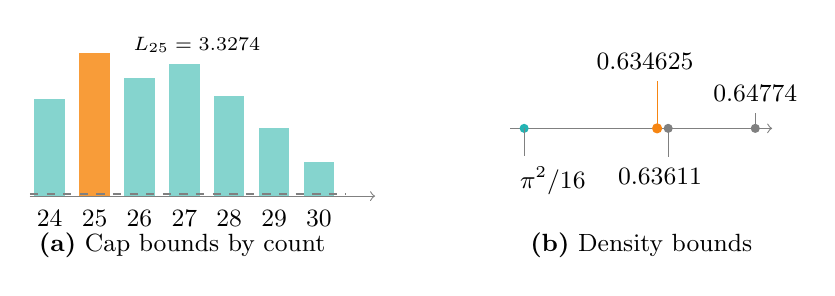
\begin{tikzpicture}[font=\small]
 \begin{scope}[x=.57cm,y=1cm]
  \draw[->,gray] (-.45,0)--(7.25,0);
  \foreach \x/\neighbornum/\level in {0/24/3.2539,1/25/3.3274,2/26/3.2880,3/27/3.3090,4/28/3.2587,5/29/3.2080,6/30/3.1538}{
   \pgfmathsetmacro{\barheight}{8*(\level-3.1)}
   \ifnum\neighbornum=25
    \fill[BurntOrange!78] (\x-.34,0) rectangle (\x+.34,\barheight);
   \else
    \fill[TealBlue!55] (\x-.34,0) rectangle (\x+.34,\barheight);
   \fi
   \node[anchor=north] at (\x,-.06) {\(\neighbornum\)};
  }
  \draw[gray,dashed] (-.44,.02644)--(6.6,.02644);
  \node[font=\scriptsize,anchor=west] at (1.65,1.92) {\(L_{25}=3.3274\)};
  \node at (2.95,-.63) {\textbf{(a)} Cap bounds by count};
 \end{scope}
 \begin{scope}[xshift=5.85cm,x=95cm,y=1cm]
  \draw[->,gray] (.000,.86)--(.035,.86);
  \fill[TealBlue] (.00185,.86) circle[radius=1.65pt];
  \draw[gray] (.00185,.86)--(.00185,.51);
  \node[anchor=north west] at (.000,.49) {\(\pi^2/16\)};
  \fill[BurntOrange] (.019625,.86) circle[radius=1.85pt];
  \draw[BurntOrange] (.019625,.86)--(.019625,1.46);
  \node[anchor=south] at (.018,1.48) {\(0.634625\)};
  \fill[gray] (.02111,.86) circle[radius=1.65pt];
  \draw[gray] (.02111,.86)--(.02111,.49);
  \node[anchor=north] at (.020,.47) {\(0.63611\)};
  \fill[gray] (.03274,.86) circle[radius=1.65pt];
  \draw[gray] (.03274,.86)--(.03274,1.06);
  \node[anchor=south] at (.03274,1.08) {\(0.64774\)};
  \node at (.0175,-.63) {\textbf{(b)} Density bounds};
 \end{scope}
\end{tikzpicture}
\caption{Updated cap and density bounds.
(a) The certified values \(L_M\) of \cref{tab:levels},
drawn from the baseline \(3.1\). The dashed line is the
threshold \(9\pi^2/8-8\). The largest value is now at
twenty-five neighbours. (b) The \(D_4\) density, the
present upper bound, the three-point bound \cite{CdLS22},
and the linear programming bound \cite{CE03}.}
\label{fig:levels}
\end{figure}
